% Created 2022-01-23 Вс 01:12
% Intended LaTeX compiler: xelatex
\documentclass[11pt]{article}
\usepackage{graphicx}
\usepackage{longtable}
\usepackage{wrapfig}
\usepackage{rotating}
\usepackage[normalem]{ulem}
\usepackage{amsmath}
\usepackage{amssymb}
\usepackage{capt-of}
\usepackage{hyperref}
\usepackage[utf8x]{inputenc}
\usepackage[T2A]{fontenc}
\usepackage[russian, english]{babel}
\babelfont{rm}{Droid Serif}
\babelfont{sf}{Droid Sans}
\let\oldsection\section
\renewcommand\section{\pagebreak\oldsection}
\author{Андрей Люнгрин, Иван Наумов, Тимофей Меньшиков}
\date{22 Января 2022}
\title{Инженерная книга\\\medskip
\large Команда с остроумным названием}
\hypersetup{
 pdfauthor={Андрей Люнгрин, Иван Наумов, Тимофей Меньшиков},
 pdftitle={Инженерная книга},
 pdfkeywords={},
 pdfsubject={},
 pdfcreator={Emacs 27.2 (Org mode 9.6)}, 
 pdflang={English}}
\begin{document}

\maketitle
\tableofcontents


\section{Команда}
\label{sec:org6a2a280}
\subsection{Андрей Люнгрин}
\label{sec:orgb06aee4}
\begin{center}
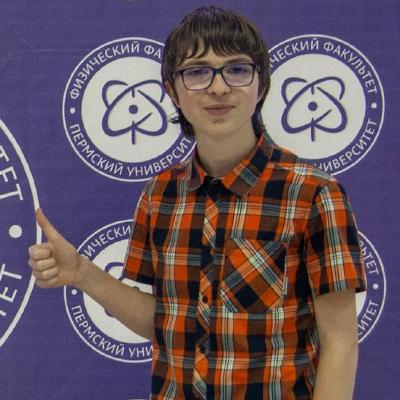
\includegraphics[width=100]{./images/andrey.jpeg}
\end{center}

\textbf{Специализация}: программирование микроконтроллеров
\subsection{Иван Наумов}
\label{sec:orge2032dd}
\begin{center}
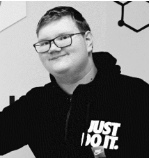
\includegraphics[width=100]{./images/ivan.jpg}
\end{center}

\textbf{Специализация}: 3d-моделирование, сборка
\subsection{Тимофей Меньшиков}
\label{sec:orga6bceb9}
\textbf{Специализация}: компьютерное зрение
\section{Общее описание робота}
\label{sec:orgea5ec12}
\begin{center}
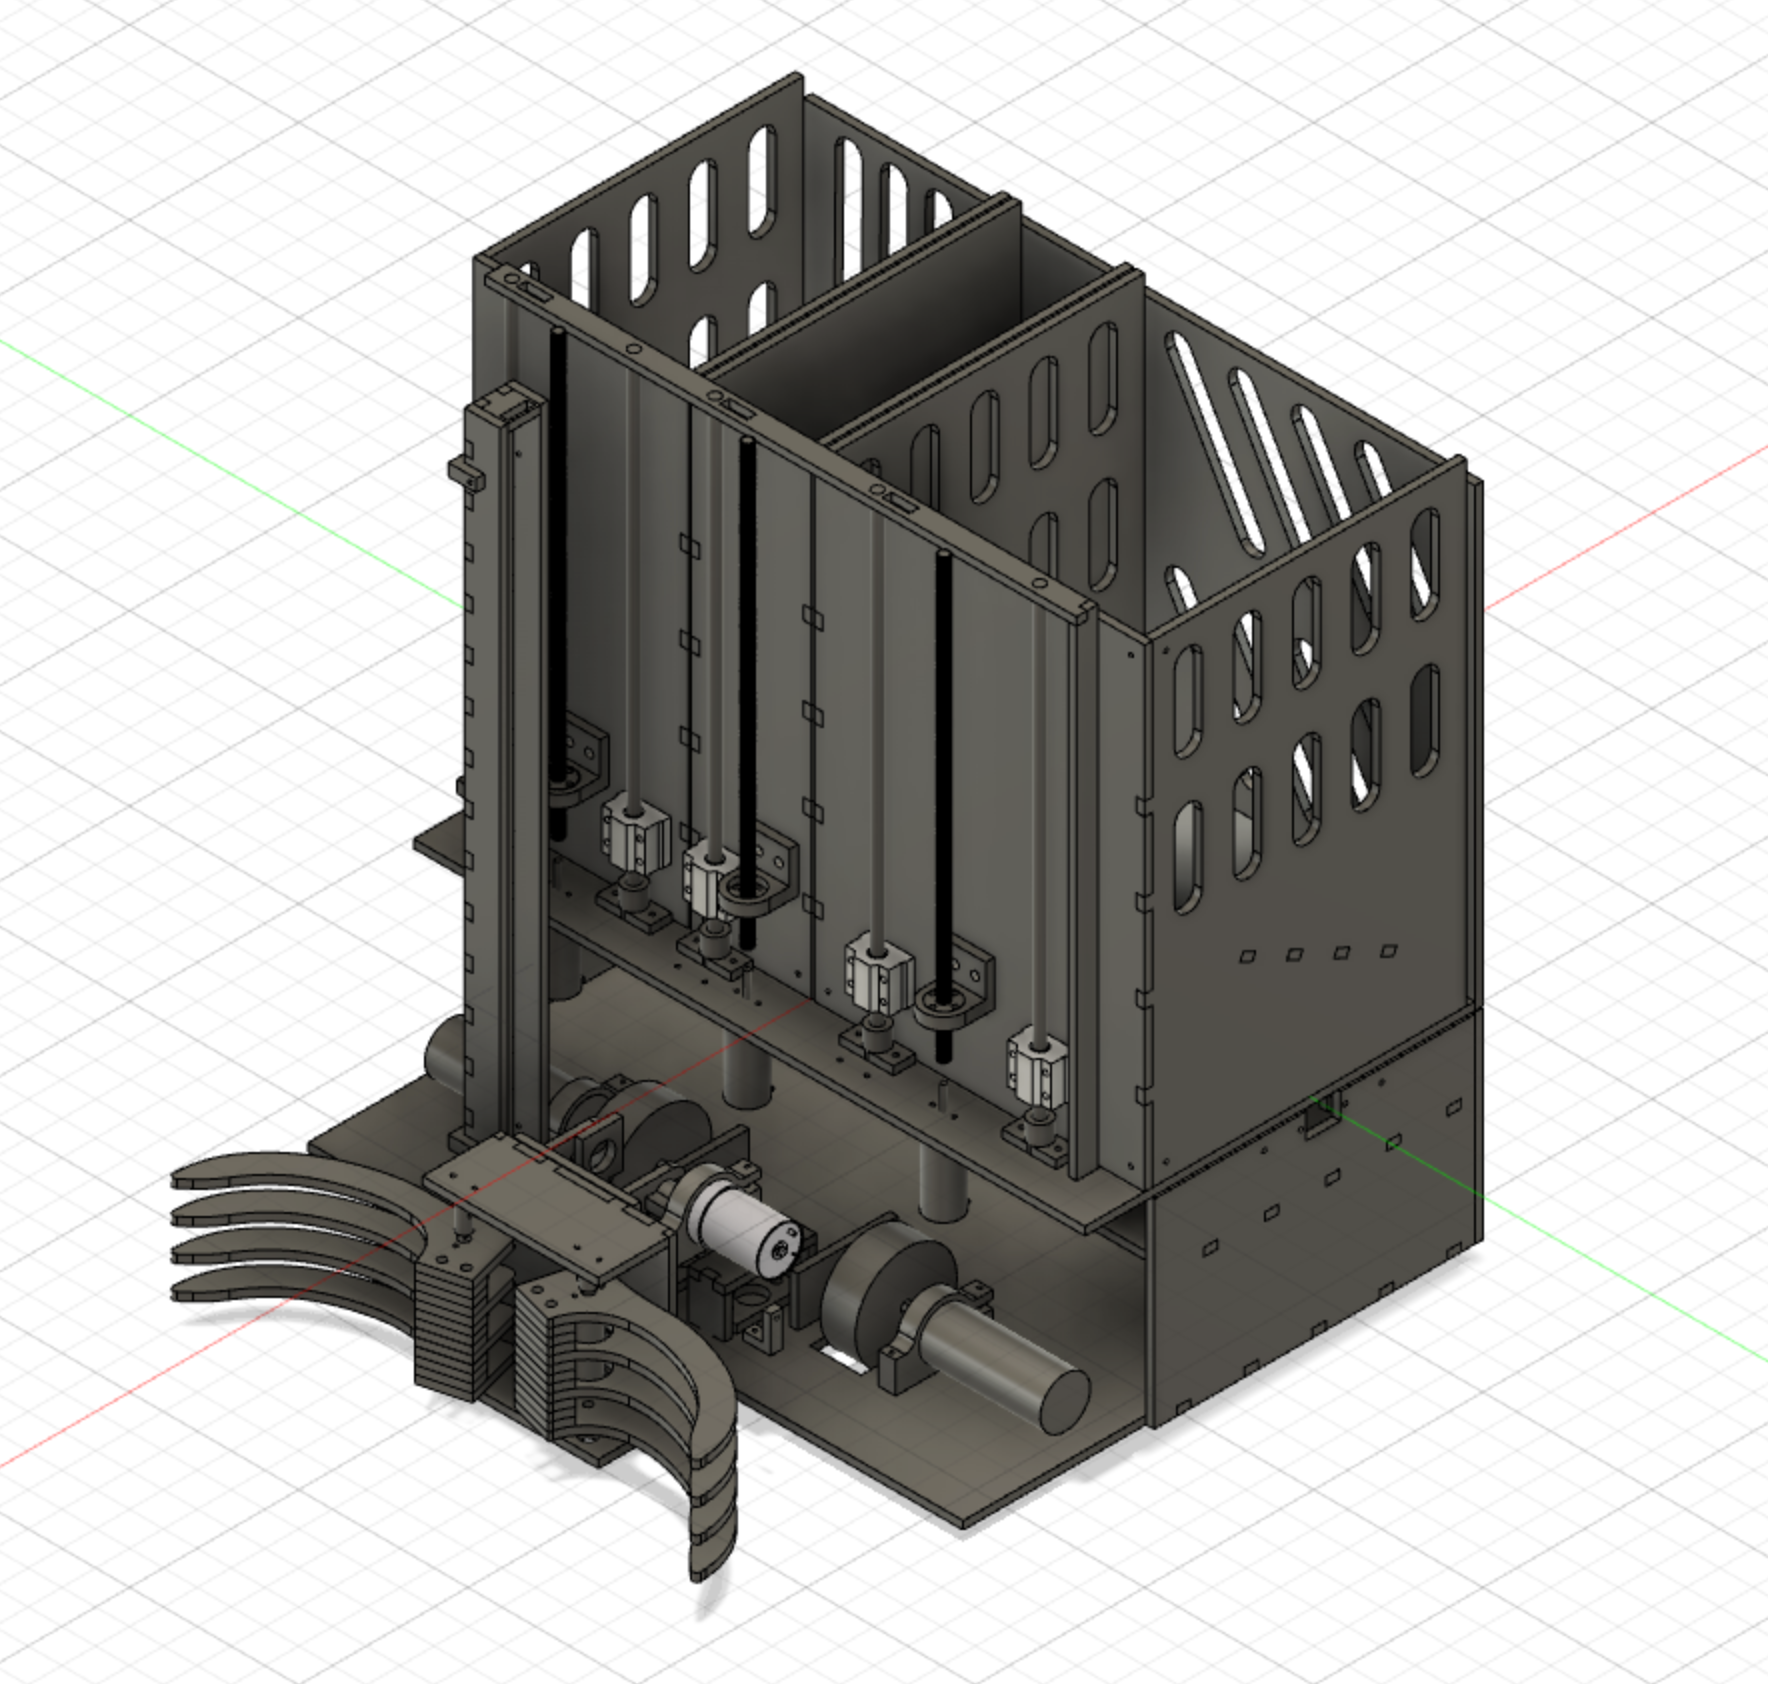
\includegraphics[width=400]{./images/robot-front-view.png}
\end{center}

Робот представляеть из себя колёсную платформу с подъёмной клешнёй спереди и тремя ящиками сзади. Размеры: ширина - 500 мм, высота - 550 мм, глубина - 496 мм.
Все структурные элементы кормуса выполнены из фанеры толщиной 6 мм. Для получения деталей использовалась технология лазерной резки. Также, некоторые элементы робота были произведены с использованием технологии трёхмерной печати, т.к. изготовление их из фанеры нецелесообразно. Такая комбинация позволяет максимально ускорить процесс производства корпуса, хотя и влечёт за собой усложнение процесса моделирование, за счёт необходимости добавления элементов стыковки деталей.
\section{Использованные САПР}
\label{sec:org6de2731}
\begin{itemize}
\item Основная работа по моделированию была проделана во \emph{Fusion 360} - современная параметрическая САПР от компании \emph{Autodesk}.
\item Небольшая часть деталей была создана во \emph{FreeCAD} - параметрическая САПР общего назначения с открытым исходным кодом.
\item Также, для создания некоторых простых деталей использовался \emph{OpenSCAD} - открытая САПР для параметрического (не визуального) создания твердотельных трёхмерных объектов.
\end{itemize}
\section{Привод}
\label{sec:org3877299}
Перемешение робота обеспечивается за счёт двух двигателей постоянного тока с редукторами. Нами были выбраны двигатели \emph{TETRIX® MAX TorqueNADO® Motor}, из-за их высокой тяги и скорости. Другим плюсом данного варианта является наличие встроенного квадратурного инкременатльного энкодера, что существенно упрощает его интеграцию в систему.

Двигатели подключены к колёсам диаметром 76 мм. Для снятия нагрузки с вала дивгателя, колёса опираются с другой стороны на подшипник. Колёса расположены внутри платформы робота, на расстоянии 17 мм. Это необходимо для увеличения скорости поворота.

В задней части платформы закреплены две шариковые опоры.
\section{Логика работы}
\label{sec:orge87443f}
Робот был спроектирован с целью минимизации количества поездок до точки сброса. Из этого следует решение хранить собранный мусор внутри робота, что, при идеальных обстоятельствах, сводит количество перемещений до точки сброса до одного - для финальной выгрузки.

Для достижения данной цели, в роботе предусмотрены три ящика. Конструкция ящика представляет из себя три боковых стенки, и дно, расположенное под наклоном. Все три ящика закрыты сзади одной общей стенкой, которая не даёт собранному мусору вывалиться. Каждый ящика оснащён подъёмной системой, которая позволяет поднять ящик выше задней стенки. Таким образом, ящик окажется открыт, и собранный мусор, за счёт скошенного дна упадёт из ящика.
Ящики спроектированы так, что любой тип мусора может поместиться в подходящий ящик, вне зависимости от его ориентации.

Для забора мусора, в передней части робота расположен захват. Его максимальный размах - 370 мм, что существенно упрощает логику захвата за счёт того, что это даёт нам возможность захватить любой предмет, вне зависимости от его ориентации, без какой-либо подстройки. Для обеспечения загрузки захваченных предметов в ящик, захват прикреплён к механизму, который позволяет поднять его выше уровня ящиков, а после этого - перевернуть его так, что предмет окажется над ящиком.

Сортировка мусора по ящикам осуществляется за счёт перемещения всей сборки ящиков в стороны, так, что нужный ящик оказывается по центру, т.е. в зоне сброса предмета захватом.
\section{Кинематика}
\label{sec:orgeab545d}
Подъём ящикаов и захвата реализован за счёт линейных направляющих и ходового винта, который приводится в движение двигателем постоянного тока.

Перемещение ящиков в стороны реализовано с использованием зубчатой рейки и шестерни, которая также приводится в движение двигателем постоянного тока.
\section{Электронника}
\label{sec:org85b2dec}
Всю электронную часть робота можно разделить на \emph{силовую} и \emph{управляющую}.

\emph{Силовой} блок, как может быть понятно из названия, отвечает за управление двигателями. Он включает в себя 5 плат драйверов двигателей постоянного тока, на базе чипа L298N. Данный выбор обусловлен лишь широкой доступностью таких плат, и не является оптимальным из-за низкой его энерго-эффективности (и следовательно - высокого тепловыделения), а также наличия более совершенных и компактных аналогов.

\emph{Управляющий} блок влючает в себя одноплатный компьютер \emph{Raspberry Pi 3B} и отладочную плату \emph{STM32 Nucleo} на базе микроконтроллера серии \emph{F401RE}.
\emph{Raspberry Pi} отвечает за обработку данных с камеры (компьютерное зрение), а также планирование маршрута и принятие других высокоуровневых решений.
Микроконтроллер отвечает за получение сигналов от датчиков (концевые выключатели и энкодеры двигателей) и генерацию управляющих сигналов для двигателей.
Такое разделение необходимо потому, что \emph{Raspberry Pi} не преспособлен для точной обработки (относительно) высокочастостных входных сигналов, и не имеет средств генерации управляющих сигналов правильной формы.
Связь между контроллерами осуществляется по виртуальному последовательному порту, через USB соединение.

Силовая часть питается от \emph{NiMH} аккумулятора на 12V/3Ah. Управляющая часть питается от отдельного USB PowerBank'а.
\section{Программная часть}
\label{sec:org651214d}
\subsection{Организация}
\label{sec:org846646d}
Весь код для проекта, а также, некоторые исходники 3D-моделей находятся в \emph{git-репозитории}, размещённом на \emph{GitHub} по аддрессу \url{https://github.com/prostoiChelovek/econet-2021}.
\subsection{Микроконтроллер}
\label{sec:orgae6d461}
ПО для микроконтроллера было написано на \emph{Rust} - компилируемый язык программирования общего назначения, одной из главных особенностей которого является гарантия безопасности памяти, за счёт встроенного в компилятор механизма проверки ссылок (\emph{Borrow-checker}).
Также, для упрощения разработки, используется фреймворк \emph{RTIC} - \emph{Real-Time Interrupt-driven Concurrency}. Он предоставляет возможность создавать конкурентные задачи, планировать их выполнение, и безопасно распределять общие ресурсы между ними.
\subsubsection{Управление двигателями}
\label{sec:org96ac56b}
Двигатели управляются с помощью двух \emph{ПИД-регуляторов}. Первый отвечает за удержание заданной скорости. Его вход - реальная скорость, полученная с энкодера (см/с); выход - скорость двигателя (\% заполнения ШИМ). Как вы могли заметить, размерности входа и выхода не совпадают. Для избежания данной проблемы, входное значение скорости нормализуется в диапазон от 0\% до 100\%, где 100\% - эксперементально выявленная максимальная скорость вращения двигателя.

Второй регулятор отвечает за удержание позиции. На вход он получает текущую позицию колеса, котора также вычисляется из данных энкодера (см); на выходе мы получаем управляющее воздействие на скорость (скорость - см/с). Для согласования размерностей, входное значение нормализуется в диапазон от -1 до 1. Управляющее воздействие прибавляется к нормализованному значению текущей скорости, и данная сумма, после денормализации, устанавливается в качестве новой целевой скорости двигателя.
\end{document}